

\begingroup
\definecolor{stepfill}{HTML}{F8FAFC}
\definecolor{stepborder}{HTML}{475569}
\definecolor{arrowcol}{HTML}{64748B}
\definecolor{steptext}{HTML}{1E293B}

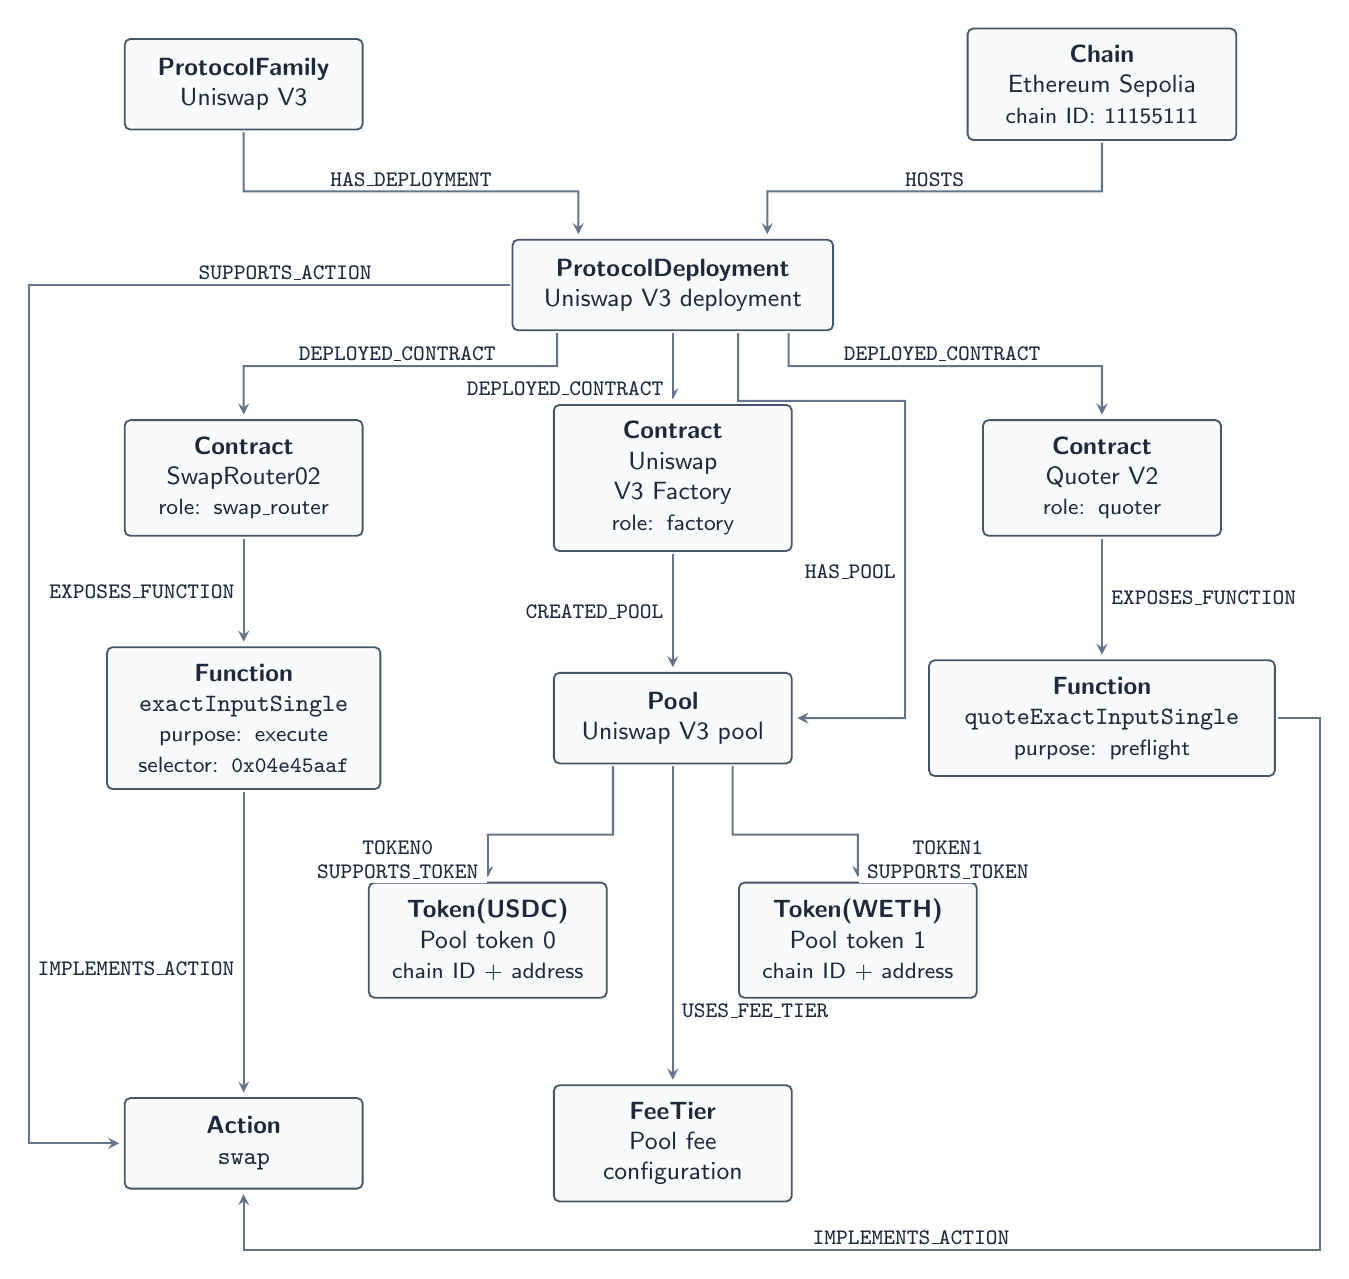
\begin{tikzpicture}[
    >=stealth,
    graphnode/.style={
        draw=stepborder,
        fill=stepfill,
        text=steptext,
        rounded corners=2pt,
        line width=0.65pt,
        text width=2.67cm,
        minimum height=1.15cm,
        inner xsep=5pt,
        inner ysep=6pt,
        outer sep=0pt,
        align=center,
        font=\sffamily\fontsize{9}{11}\selectfont
    },
    edge/.style={
        ->,
        draw=arrowcol,
        line width=0.76pt,
        rounded corners=0pt,
        shorten <=1pt,
        shorten >=2pt
    },
    rel/.style={
        fill=white,
        text=steptext,
        inner xsep=3pt,
        inner ysep=1.5pt,
        align=center,
        font=\ttfamily\fontsize{7.6}{8.9}\selectfont
    }
]

% --- Top row -----------------------------------------------------
\node[graphnode] (family) at (-5.45,0)
    {\textbf{ProtocolFamily}\\Uniswap V3};
\node[graphnode, text width=3.06cm] (chain) at (5.45,0)
    {\textbf{Chain}\\Ethereum Sepolia\\{\footnotesize chain ID: 11155111}};

% --- Deployment --------------------------------------------------
\node[graphnode, text width=3.72cm] (deployment) at (0,-2.55)
    {\textbf{ProtocolDeployment}\\Uniswap V3 deployment};

% --- Contract layer ---------------------------------------------
\node[graphnode] (router) at (-5.45,-5.0)
    {\textbf{Contract}\\SwapRouter02\\{\footnotesize role: swap\_router}};
\node[graphnode] (factory) at (0,-5.0)
    {\textbf{Contract}\\Uniswap V3 Factory\\{\footnotesize role: factory}};
\node[graphnode] (quoter) at (5.45,-5.0)
    {\textbf{Contract}\\Quoter V2\\{\footnotesize role: quoter}};

% --- Function and pool layer ------------------------------------
\node[graphnode, text width=3.12cm] (execute) at (-5.45,-8.05)
    {\textbf{Function}\\\texttt{exactInputSingle}\\{\footnotesize purpose: execute}\\{\footnotesize selector: \texttt{0x04e45aaf}}};
\node[graphnode] (pool) at (0,-8.05)
    {\textbf{Pool}\\Uniswap V3 pool};
\node[graphnode, text width=4.04cm] (quote) at (5.45,-8.05)
    {\textbf{Function}\\\texttt{quoteExactInputSingle}\\{\footnotesize purpose: preflight}};

% --- Pool resources ---------------------------------------------
\node[graphnode] (token0) at (-2.35,-10.87)
    {\textbf{Token(USDC)}\\Pool token 0 \\{\footnotesize chain ID + address}};
\node[graphnode] (token1) at (2.35,-10.87)
    {\textbf{Token(WETH)}\\Pool token 1 \\{\footnotesize chain ID + address}};

% --- Terminal nodes ---------------------------------------------
\node[graphnode] (action) at (-5.45,-13.45)
    {\textbf{Action}\\\texttt{swap}};
\node[graphnode] (fee) at (0,-13.45)
    {\textbf{FeeTier}\\Pool fee\\configuration};

% --- Top relationships: mirrored orthogonal bends --------------
\draw[edge]
    (family.south) -- (-5.45,-1.36)
    -- node[rel, above, pos=0.50] {HAS\_DEPLOYMENT} (-1.20,-1.36)
    -- ([xshift=-1.20cm]deployment.north);
\draw[edge]
    (chain.south) -- (5.45,-1.36)
    -- node[rel, above, pos=0.50] {HOSTS} (1.20,-1.36)
    -- ([xshift=1.20cm]deployment.north);

% --- Contract ownership: mirrored routing lanes ----------------
\draw[edge]
    ([xshift=-1.47cm]deployment.south) -- (-1.47,-3.58)
    -- node[rel, above, pos=0.51] {DEPLOYED\_CONTRACT} (-5.45,-3.58)
    -- (router.north);
\draw[edge]
    (deployment.south) -- node[rel, left, pos=0.78]
    {DEPLOYED\_CONTRACT} (factory.north);
\draw[edge]
    ([xshift=1.47cm]deployment.south) -- (1.47,-3.58)
    -- node[rel, above, pos=0.49] {DEPLOYED\_CONTRACT} (5.45,-3.58)
    -- (quoter.north);

% --- Pool ownership: dedicated inter-column corridor -----------
\draw[edge]
    ([xshift=0.83cm]deployment.south) -- (0.83,-4.02)
    -- (2.95,-4.02)
    -- node[rel, left, pos=0.54] {HAS\_POOL} (2.95,-8.05)
    -- (pool.east);

% --- Direct contract/function and factory/pool connections ------
\draw[edge]
    (router.south) -- node[rel, left, pos=0.50]
    {EXPOSES\_FUNCTION} (execute.north);
\draw[edge]
    (factory.south) -- node[rel, left, pos=0.50]
    {CREATED\_POOL} (pool.north);
\draw[edge]
    (quoter.south) -- node[rel, right, pos=0.50]
    {EXPOSES\_FUNCTION} (quote.north);

% --- Resource relationships: symmetrical orthogonal bends ------
\draw[edge]
    ([xshift=-0.76cm]pool.south) -- (-0.76,-9.53)
    -- (-2.35,-9.53)
    -- node[rel, left, pos=0.52] {TOKEN0\\SUPPORTS\_TOKEN}
       (token0.north);
\draw[edge]
    ([xshift=0.76cm]pool.south) -- (0.76,-9.53)
    -- (2.35,-9.53)
    -- node[rel, right, pos=0.52] {TOKEN1\\SUPPORTS\_TOKEN}
       (token1.north);
\draw[edge]
    (pool.south) -- node[rel, right, pos=0.77]
    {USES\_FEE\_TIER} (fee.north);

% --- Action relationships: own channels, no node crossings ------
\draw[edge]
    (execute.south) -- node[rel, left, pos=0.58]
    {IMPLEMENTS\_ACTION} (action.north);

\draw[edge]
    (deployment.west) -- node[rel, above, pos=0.47]
    {SUPPORTS\_ACTION} (-8.18,-2.55)
    -- (-8.18,-13.45)
    -- (action.west);

\draw[edge]
    (quote.east) -- (8.22,-8.05)
    -- (8.22,-14.80)
    -- node[rel, above, pos=0.38] {IMPLEMENTS\_ACTION} (-5.45,-14.80)
    -- (action.south);

\end{tikzpicture}
\endgroup
